\documentclass[../main.tex]{subfiles}
\begin{document}
%\chapter{Landau Zener}\label{ch:LZ}
The Landau-Zener model describes the response of the magnetization of a 2-level spin system, under the action of a slowly reversing external magnetic field at zero temperature \cite{landau1932theorie,zener1932non,de1997theory}. Consider, the following single spin-1/2 Hamiltonian as an example:
\begin{equation}
H_{LZ}(t)=-\Gamma \sigma_x -c t \sigma_z, \label{eq:lz1}
\end{equation}
where $\Gamma$ sets the scale of the splitting between the two energy levels, and $c$ is the sweep rate of the applied magnetic field, i.e $H(t)=ct$. Thus for a field switching its value from $-H_0$ to $H_0$ in time $T$, $c=\Delta H/T= 2H_0/T$.

Now, for large negative times $t$, and $\abs{H(t)} \geq \abs{\Gamma}$, $H_{LZ}(t)\approx ct \sigma_z$. Thus, the spin-down state, $\ket{\downarrow}$, is close to the ground state of the Hamiltonian, as $ct \sigma_z \ket{\downarrow}=-ct \ket{\downarrow}$. As $t$ goes to infinity, $H_{LZ}(t)\approx -ct \sigma_z$, so that the ground state now lies close to the spin up state, $\ket{\uparrow}$, as $-ct \sigma_z \ket{\uparrow}=-ct \ket{\uparrow}$. According to the quantum adiabatic theorem, the state of the system should always lie close to the instantaneous ground state of the Hamiltonian $H(t)$, if one starts with the ground state and if the field is changed slowly enough. However, there is a finite probability that the state transits to a higher excited level during the sweep. The probability, $p'$, for this non-adiabatic transition (Landau-Zener tunnelling), as given by the Landau-Zener formula, is
\begin{equation}
p'=\exp(\frac{-\pi {\Gamma}^2}{\hbar c}) . 
\end{equation}
Therefore, the probability, $p$, that the state of the system follows the instantaneous ground state of the Hamiltonian adiabatically, by changing the magnetization state of the system, in accordance to the reversing field, $H(t)$, is \cite{landau1932theorie,zener1932non,de1997theory,miyashita1995dynamics}.
\begin{equation}
p=1-p'=1-\exp(\frac{-\pi {\Gamma}^2}{c}) ,   \label{eq:lz2}
\end{equation}
where $\hbar=1$.\\
If the minimum energy splitting between the ground state and the first excited state of the Hamiltonian at the anti-crossing is denoted by $\Delta_{min}$, then it can be observed that $\Delta_{min}= 2 \Gamma$. Thus, in terms of $\Delta_{min}$, Eq.~(\ref{eq:lz3}) becomes 
\begin{equation}
p=1-\exp(\frac{-\pi {\Delta_{min}}^2}{4c}) .   \label{eq:lz3}
\end{equation}

The deviation from the ground state occurs at $H \approx 0$, with a probability $p'$, and is accompanied by a step in the magnetization. This step depends on both the energy splitting  $\Delta_{min}$, and the sweep rate $c$ \cite{de1997theory}.\\
\begin{figure}[H]
\centering 
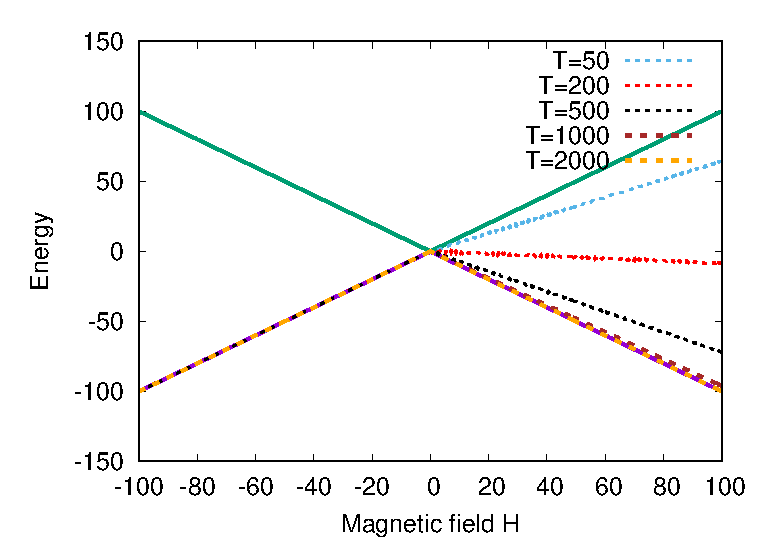
\includegraphics[scale=0.8]{EnergySpec_1spin_H100.eps}
\caption{Energy spectrum for single qubit Hamiltonian in Eq.~(\ref{eq:lz1}), with energy expectation values of the instantaneous state of the system with different sweeping times. The parameters used are $\Gamma=0.5$, $H_0=100$.}
\label{fig:lz1}
\end{figure}

For a simple 2-level system where $\Gamma$ is chosen to be 0.5 and the field is swept from a value from -100 to 100, Fig.~(\ref{fig:lz1}) gives the energy spectra for the Hamiltonian in Eq.~(\ref{eq:lz1}).
Figure~(\ref{fig:lz1}) also shows the energy expectation values corresponding to the instantaneous state of the system for different times $T$ chosen for sweeping the field. As is evident from the figure, the probability of the state of the system staying close to the ground state increases with decreasing speed (increasing $T$), as expected from Eq.~(\ref{eq:lz2}). For a sweeping time of $T$=500, Fig.~(\ref{fig:lz2}) shows the instantaneous magnetization state of the system.
\begin{figure}[H]
\centering 
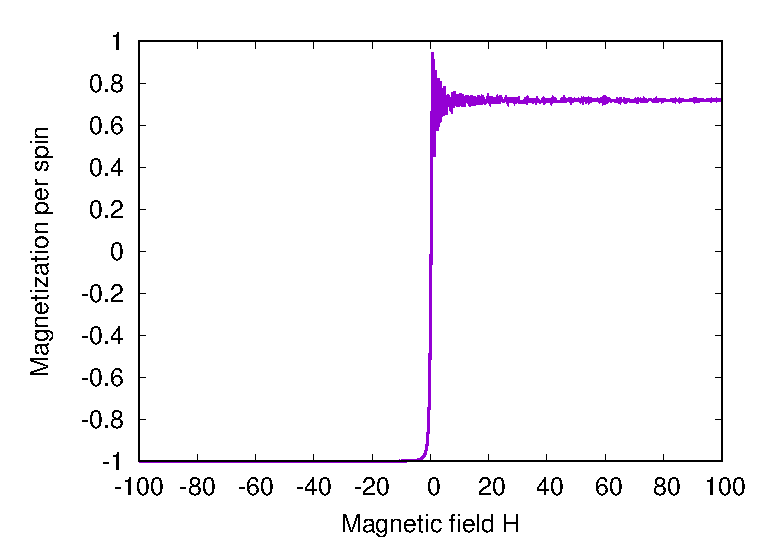
\includegraphics[scale=0.8]{Magnetization_500.eps}
\caption{Instantaneous magnetization of the system state for $\Gamma=0.5$, $H_0=100$, $T$=500 and $c$=0.4.}
\label{fig:lz2}
\end{figure}
Comparing Figs. (\ref{fig:lz1}) and (\ref{fig:lz2}), it can be observed that the step in the magnetization corresponds to the position of the anti-crossing between the ground state and the first excited state in the energy spectrum.\\

For verifying Eq.~(\ref{eq:lz2}), the overlap of the resulting state was computed with the ground state of the Hamiltonian, for different sweeping times. Figure~(\ref{fig:lz3}) shows the result obtained.\\

From Eq.~(\ref{eq:lz2}), $p=1-e^{-aT}$, where $a={\pi \Gamma^2/2H_0}$. For the chosen parameters, $a$ was calculated to be $3.926 \times 10^{-3}$. This value was found to be in reasonable agreement with the value $3.198 \times 10^{-3}$, obtained for the fitting parameter in Fig.~(\ref{fig:lz3}). The difference in the two values could be arising due to the magnetic field not being large enough, as is required by the theory.

\begin{figure}[H]
\centering 
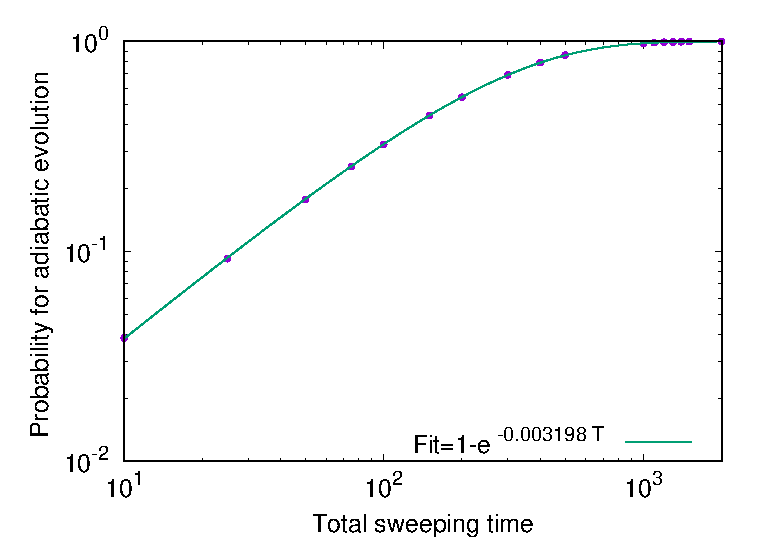
\includegraphics[scale=0.8]{Prob_1spin_H100.eps}
\caption{Probability for adiabatic evolution as a function of different sweep times for $\Gamma=0.5$.}
\label{fig:lz3}
\end{figure}


Although in both Quantum annealing and the Landau-Zener model one deals with time dependent Hamiltonians, and the main task consists of studying the evolution of the state of the system under its action, there are two major points of difference. The Landau-Zener formula is applicable to 2-level systems, and the process of reversing the magnetic field is ideally carried over an infinite amount of time. On the other hand, the Ising Hamiltonian considered for quantum annealing generally consists of more than two energy levels, and the evolution is carried out for a limited time, i.e. from $s$=0 to $s$=1 in terms of the annealing parameter: $s=t/T_A$, where $T_A$ is the total annealing time.

Despite these differences, the Landau-Zener formula can be used to predict the probability of an adiabatic evolution for an Ising model, by making use of some approximations \cite{miyashita1996observation}. The Ising model in a transverse field involving $N$ variables is one of the simplest microscopic models for uniaxial magnets. Consider, for example, the Hamiltonian
\begin{equation}
H=-J \sum \limits_{\langle i,j\rangle} \sigma_i^z \sigma_j^z - \Gamma \sum \limits_i \limits^N \sigma_i^x -H(t) \sum \limits_i \limits^N\sigma_i^z, \label{eq:lz4}
\end{equation} 
where set $\langle i,j \rangle$ defines the interactions between pairs of spins in the cluster. For a uniaxial magnet, only the lowest two levels are important for the adiabatic motion of the ground state. The scattering from the ground state to the first excited state occurs only when these levels come close, at the point of anti-crossing, i.e. around $H$=0. The dependence of energy on $H$ around the anti-crossing is expected to be approximately expressed  as the eigenvalue of the two level system:
\begin{equation}
(M_0H\sigma^z-\Gamma \sigma^x)\ket{\psi}=E(H)\ket{\psi}, \label{eq:lz6}
\end{equation}
where $M_0$ is a saturated magnetization at high field. In the case of a strong uniaxial magnet, $M_0=N$. The probability for the system state to follow the ground state adiabatically then becomes
\begin{equation}
p_N=1-\exp(\frac{-\pi {\Delta_{min}}^2}{4Nc}). \label{eq:lz5}
\end{equation}
Choosing a two spin system, with $\Gamma=0.5$, $J=3$, and $H_0=100$, Fig.~(\ref{fig:lz4}) shows the energy spectrum as a function of the magnetic field.
\begin{figure}[H]
\centering 
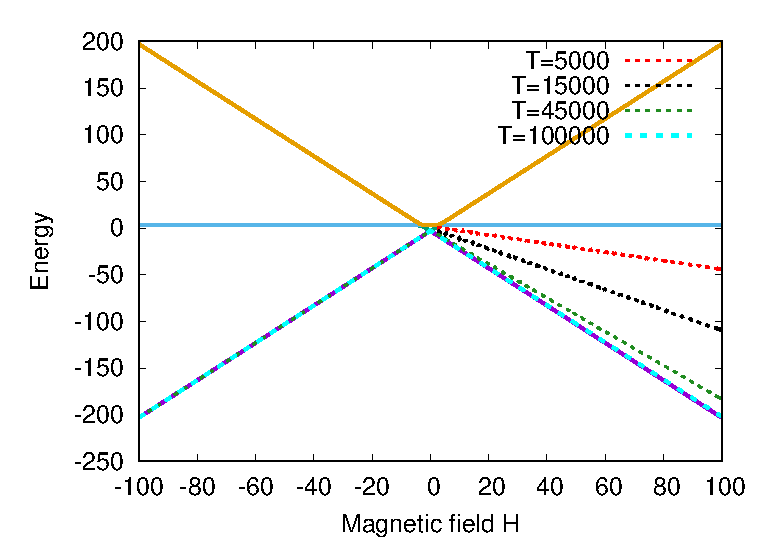
\includegraphics[scale=0.8]{EnergySpectrum_H100.eps}
\caption{Energy spectrum for two spin Hamiltonian in Eq.~(\ref{eq:lz4}), with energy expectation value of the instantaneous state of the system with different sweeping times. The parameters used are $\Gamma=0.5$, $J=3$, $H_0=100$.}
\label{fig:lz4}
\end{figure}

\begin{figure}[H]
  \centering
    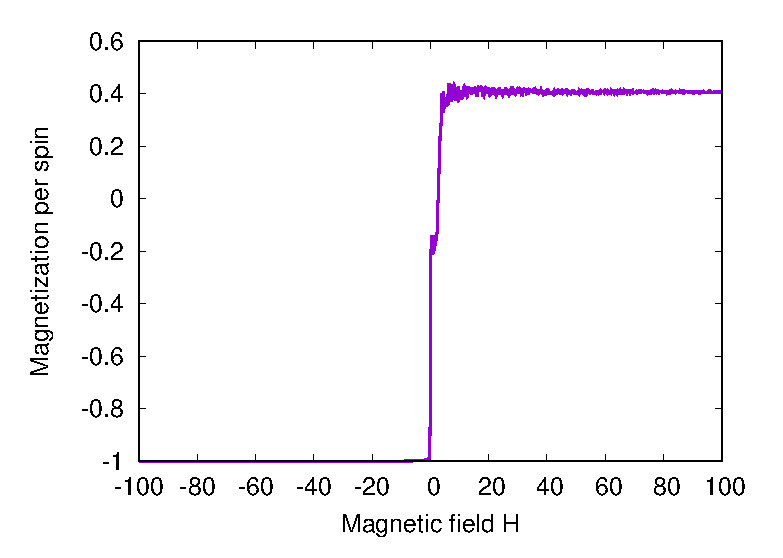
\includegraphics[scale=0.8]{Mag_13_H100.eps}
    \caption{Instantaneous magnetization of the system state for $\Gamma=0.5$, $H_0=100$, $T$=10000 and $c$=0.02.}
  \label{fig:lz5}
 \end{figure}

Figures~(\ref{fig:lz5}) and (\ref{fig:lz6}) show the instantaneous magnetization values for two different sweep rates, corresponding to $T$=10000 and $T$=20000 respectively. Similar to the case of a single spin Hamiltonian, the steps in the magnetization values correspond to the position of anti-crossing between the energy levels of the spectrum, in this case as well. Other than the first step in the magnetization at $H \approx 0$, in this case, the second step corresponds to the anti-crossing between the first and the second excited state of the Hamiltonian.

 \begin{figure}[H]
  \centering
    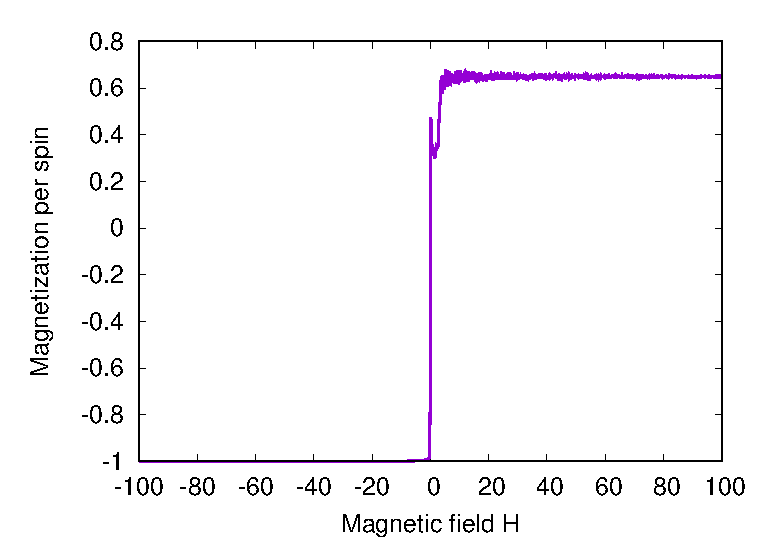
\includegraphics[scale=0.8]{Mag_9_H100.eps}
    \caption{Instantaneous magnetization of the system state for $\Gamma=0.5$, $H_0=100$, $T$=20000 and $c$=0.01.}
  \label{fig:lz6}
\end{figure}

\begin{figure}[H]
\centering 
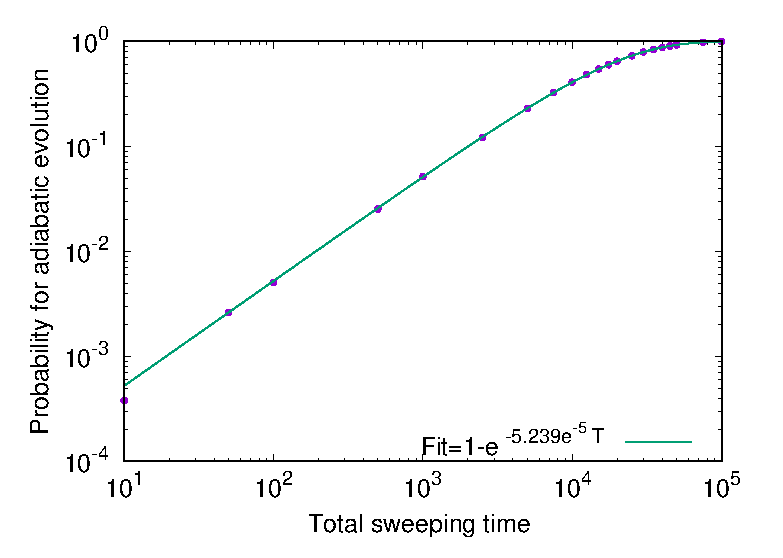
\includegraphics[scale=0.8]{Probability_H100.eps}
\caption{Probability for adiabatic evolution as a function of different sweep times for $\Gamma=0.5$ and $J=3$.}
\label{fig:lz7}
\end{figure}

On increasing the total time for sweeping the field, i.e. decreasing the sweeping speed, the probability of staying in the ground state, by changing the state of magnetization should increase. This can be confirmed by comparing Figs. (\ref{fig:lz5}) and (\ref{fig:lz6}).

Finally, for verifying Eq.~({\ref{eq:lz5}}) the overlap of the resulting state with the ground state is computed for different times. Results obtained are shown in Fig.~(\ref{fig:lz7}). 

The value of the minimum gap, $\Delta_{min}$ obtained was 0.162, which results in $a={\pi \Delta_{min}^2/8 \Delta H}= 5.182 \times 10^{-5}$. The value of the fitting function obtained in Fig.~(\ref{fig:lz7}) is $5.239 \times 10^{-5}$. Thus, the Landau-Zener formula can be extended to the $N$-spin Ising Hamiltonian with the approximations.\\

Equation~(\ref{eq:lz5}) will be used again as a check for adiabatic evolution in the subsequent chapters.


\end{document}